\documentclass[french]{article}
\usepackage[T1]{fontenc}
\usepackage[utf8]{inputenc}
\usepackage{lmodern}
\usepackage[a4paper]{geometry}
\usepackage{babel}
\usepackage{amsmath}
\usepackage{amsfonts}
\usepackage{amssymb}
\usepackage{wrapfig}
\usepackage{graphicx}
\author{Badr YOUBI IDRISSI}
\title{Mini projet : évolution des tâches sur la matrice d'Heisenhower}
\begin{document}
\maketitle
\section{Introduction et Modélisation}

    La matrice d'Heisenhower est un outil d'organisation qui classe les tâches en fonction de leur 
    importance et leur urgence. Ce qui aide à se fixer des priorités. Le but de ce modèle est d'étudier
    l'évolution du travail restant à faire en fonction du temps, de l'urgence et de l'importance d'une tache.
    
    Pour pouvoir utiliser des EDP je me place dans un cadre continu : l'espace $\Omega$ est l'espace (urgence, importance). Une tache est représenté par 
    une gaussienne de moyenne $(\mu_x,\mu_y)$ avec $\mu_x$ l'urgence de la tache et $\mu_y$ son importance.
    Ceci peut être justifié en pensant une tache comme plusieurs sous-taches d'importance et d'urgence variant
    autour de la moyenne. L'écart type $\sigma$ de la tâche représente l'étalement de la tâche.

    \subsection{\'Equation}
    Soit $\Omega = [0,1]^2$,
    
    \begin{equation}\label{EDP}
        \frac{\partial u}{\partial t} + \lambda\frac{\partial u}{\partial x} + \nu.u = \rho 
    \end{equation}
    \begin{alignat*}{6}
        u \;:\; &\text{\;Densité de travail restant} \\
        \lambda \;:\; &\text{\;Vitesse de l'augmentation en urgence d'une tache}\\
        \nu \;:\; &\text{\;Efficacité} = \frac{1}{\tau(x,y)} \text{ avec } \tau(x,y) \text{ le temps caractéristique de complétion d'une tache en} \,(x,y)
    \end{alignat*}
    
    Dans ce modèle on a
    \begin{align}
        \forall(x,y)\in\Omega, \; \lambda(x,y) &= C(1+y)^2 \\
        \forall(x,y)\in\Omega, \; \nu(x,y) &= (L_4-L_1)x+(L_2-L_1)y+(L_1+L_3-L_4-L_2)xy+L_1
    \end{align}
    

    \begin{wrapfigure}{l}{0.25\textwidth}
        \begin{center}
            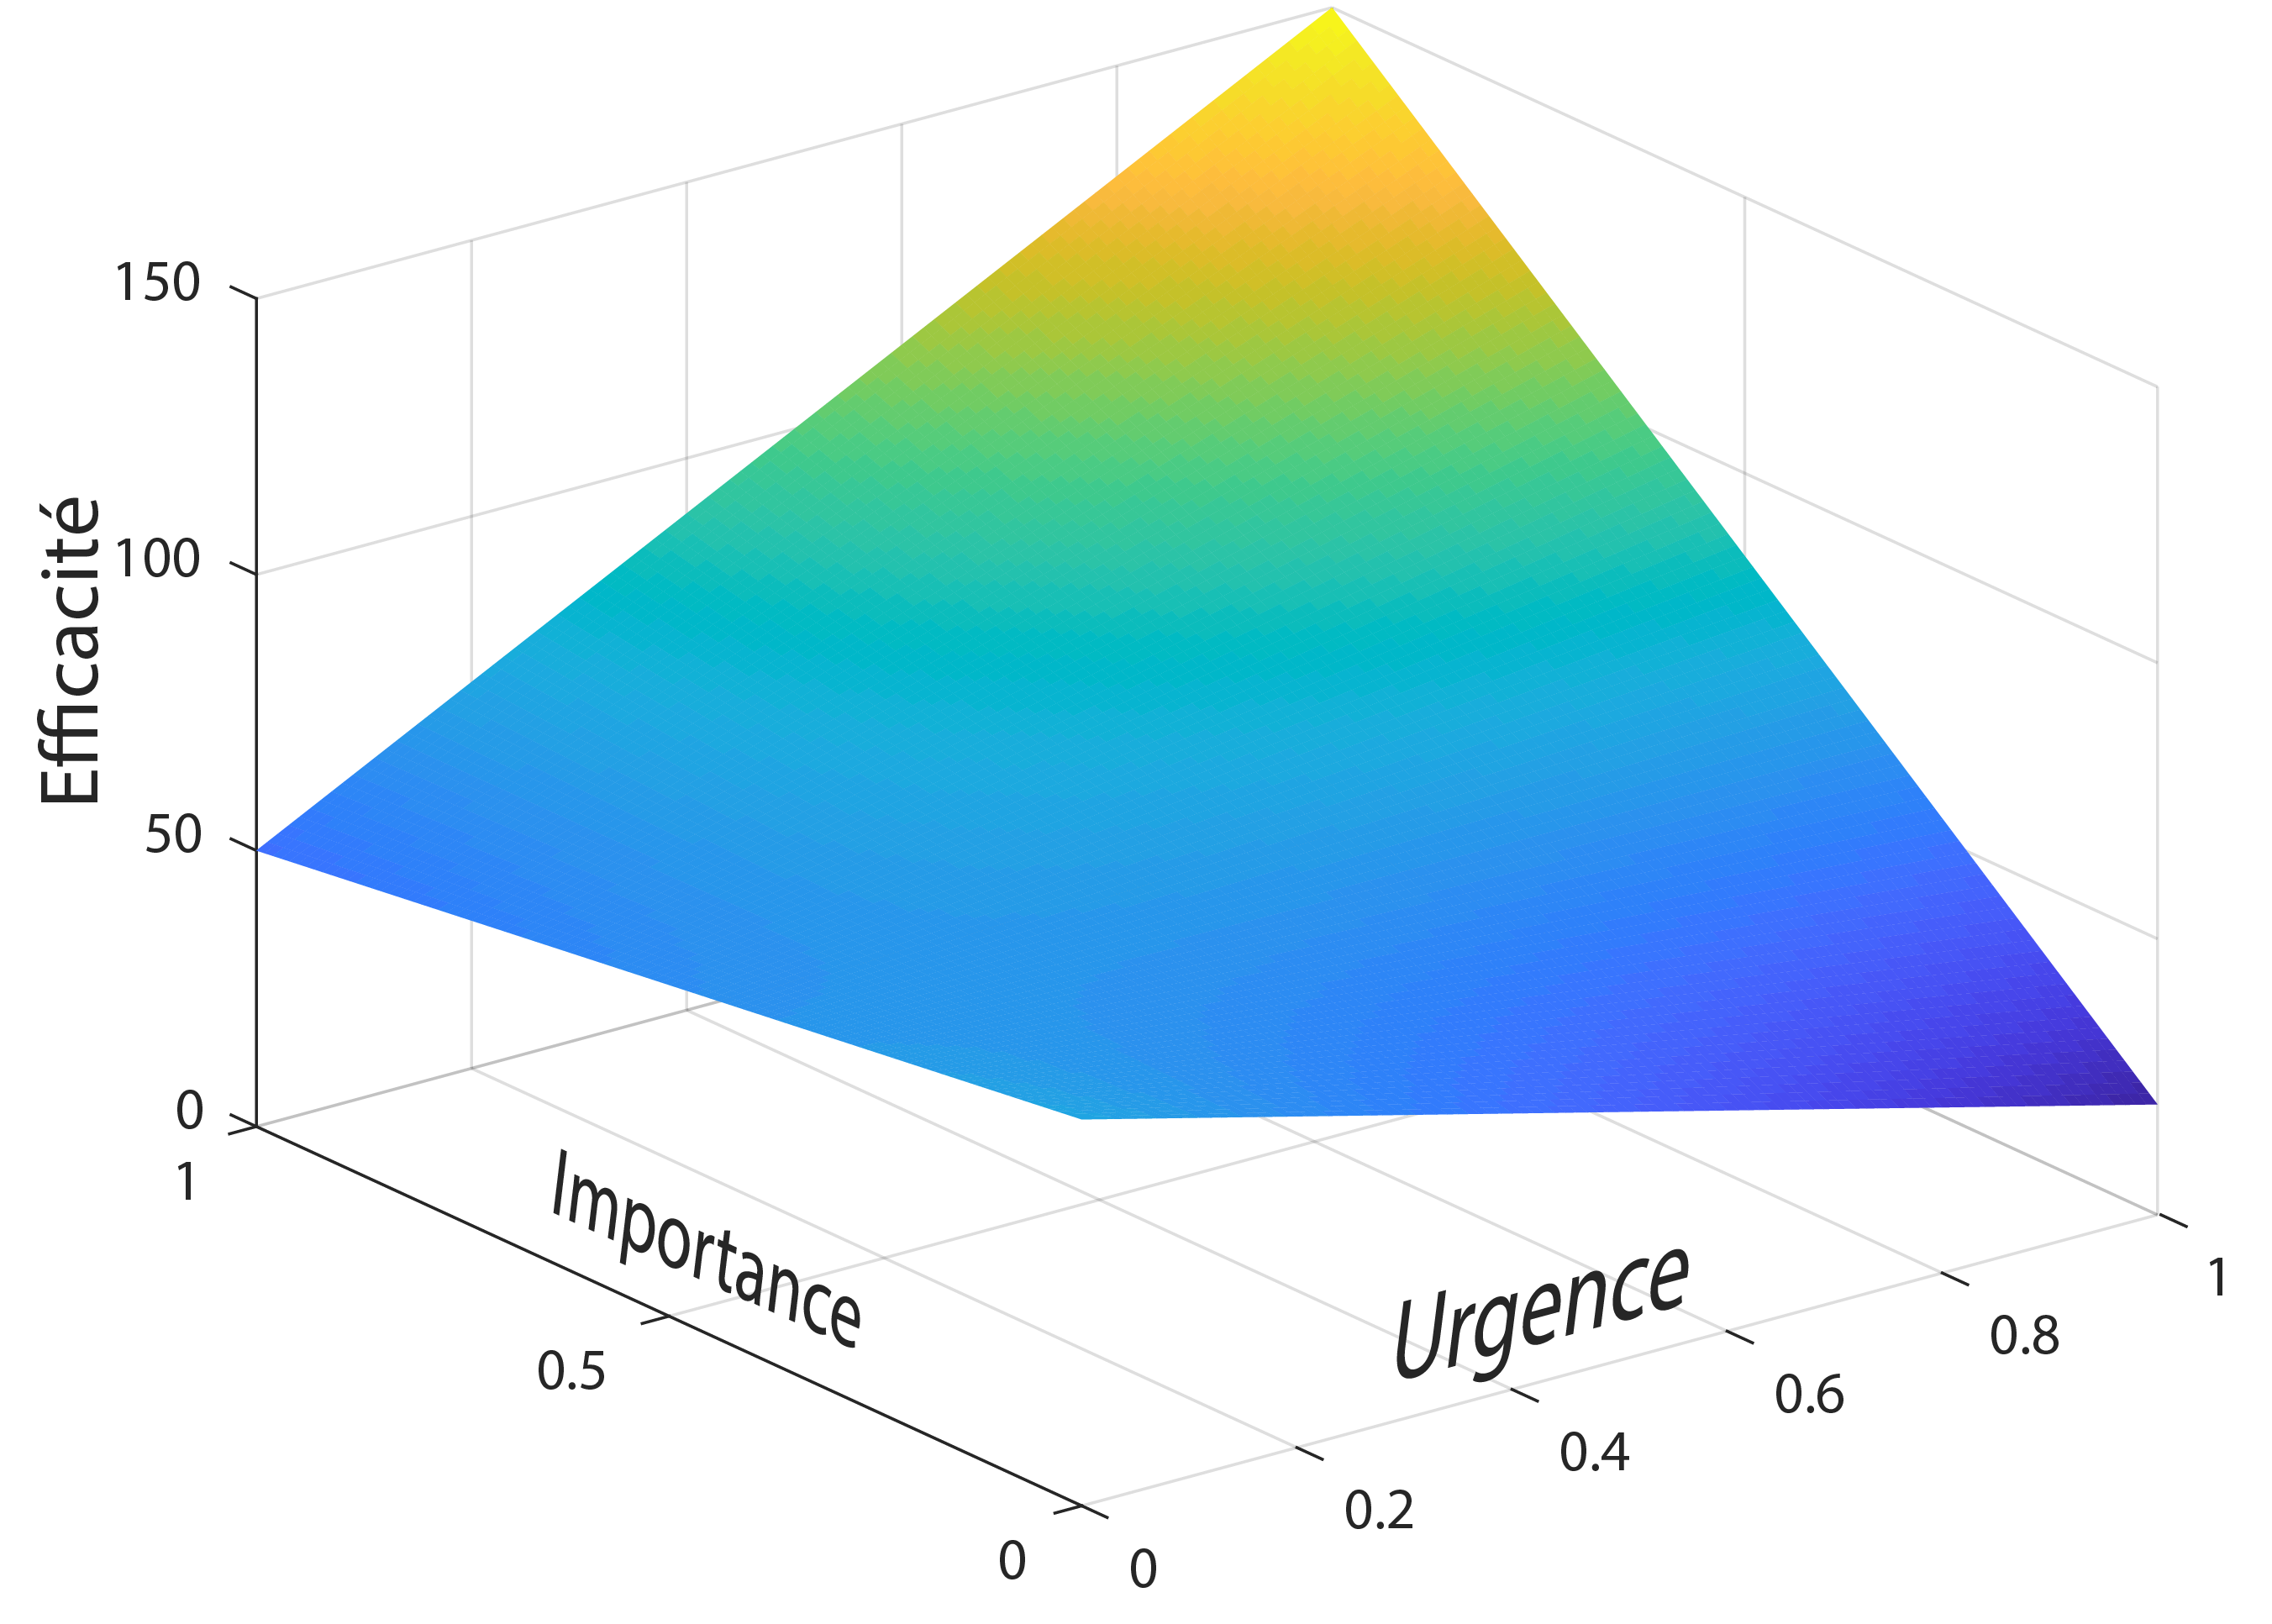
\includegraphics[width=0.23\textwidth]{Figures/Efficacite.png}
        \end{center}
    \end{wrapfigure}

    Avec $C > 0$ une constante de "convection". La fonction $\lambda$ reflète le fait que les taches importantes sont de manière générale plus urgentes que les non importantes. 
    $L_i > 0$ les valeurs de l'efficacité en $\{(0,0),(1,0),(1,1),(1,0)\}$. la fonction $\nu$ ne fait qu'interpoler continuement entre ces valeurs. Les valeurs $L_i$ caractérisent la personne qui accomplit les taches. Par exemple un grand $L_1$ relativement aux autres signifie que  la personne a une tendance à effectuer des taches non urgentes et non importantes.
    
    
    \section{Formulation Variationnelle}
    
\end{document}
